\chapter{Vektorbündel}

Betrachte $\T M$ als glatte Mannigfaltigkeit durch
	\[ \T M|_U = \pi^{-1}(U) \to \varphi(U) \times \R^m \cong U \times \R^m \]
	\[ X_p = \sum \xi^i\pdifffrac[p]{}{x^i} \mapsto \left(\varphi(p),\xi\right). \]
Fasern : $\T_pM = \pi^{-1}(p)$ $m$-dimensionaler Vektorraum und $X_p = \sum \xi^i \pdifffrac[p]{}{x^i} \mapsto \xi$ ist ein linearer Isomorphismus.

% Definition 5.1
\begin{Dfn}
  Ein \CmMark{glattes reelles Vektorbündel} vom Rang $k$ über einer glatten Mannigfaltigkeit $M$ ist eine glatte Mannigfaltigkeit $E$, der sogenannte \CmMark{Totalraum} des Bündels, zusammen mit einer glatten Abbildung $\pi \colon E \to M$, der Projektion, sodass für jedes $p \in M$ gilt:
  \begin{enumerate}[label=(\roman*)]
  \item Die Faster $E_p = \pi^{-1}(p)$ trägt die Struktur eines $k$-dimensionalen reellen Vektorraumes.
  \item Es existiert eine Umgebung $U$ von $p$ in $M$ und ein Diffeomorphismus
    \begin{align*}
      \tau \colon E|_U = \pi^{-1}(U) \to U \times \R^k,
    \end{align*}
    so dass die Einschränkung
    \begin{align*}
      \tau_p \colon E_p \to \R^k \quad ( \cong \{p\} \times \R^k)
    \end{align*}
    ein linearer Isomorphismus ist.
    Ein solches $\tau$ heißt \CmMark{B"undelkarte}.
  \end{enumerate}
\end{Dfn}

\begin{bsp}
  \begin{enumerate}[label=(\arabic*)]
  \item $E = M \times \R^k$ mit $\pi \colon E \to M, (p,x) \mapsto p$.
  \item Das Tangentialbündel $\T M$ auf $M$.
  \item Ist $E \xrightarrow{\pi} M$ ein Vektorbündel über $M$ und $U \subseteq M$ offen (oder eine Untermannigfaltigkeit), so ist $E|_U = \pi^{-1}(U)$ ein Vektorbündel über $U$.
  \end{enumerate}
\end{bsp}

Ein \CmMark{Vektorbündelmorphismus} zwischen zwei Vektorbündeln $E \xrightarrow{\pi} M$ und $E' \xrightarrow{\pi'} N$ ist eine glatte Abbildung $F \colon E \to E'$, so dass eine glatte Abbildung $f$ existiert für die das folgende Diagram kommutiert

\begin{center}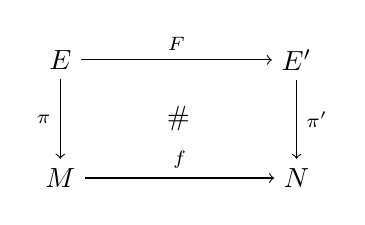
\begin{tikzpicture}
	%\draw[step=0.25,gray!15] (-6,-1) grid (6,5); \draw[step=0.5,gray!30] (-6,-1) grid (6,5); \fill (0,0) circle(0.1); %Hilfsgitter
	\node (E) at (-1.5,0.75) {$E$}; \node (E') at (1.5,0.75) {$E'$}; \node (M) at (-1.5,-0.75) {$M$}; \node (N) at (1.5,-0.75) {$N$};
	
	\draw[->] (E) --node[above,font=\scriptsize]{$F$} (E'); \draw[->] (M) --node[above,font=\scriptsize]{$f$} (N);
	\draw[->] (E) --node[left,font=\scriptsize]{$\pi$} (M); \draw[->] (E') --node[right,font=\scriptsize]{$\pi'$} (N);
	
	\node at (0,0) {$\#$};
\end{tikzpicture}\end{center}

und ferner für $p \in M$ die Abbildung $E_p \xrightarrow{F} E'_{f(p)}$ linear ist.

Gilt $M = N$ so ist ein $M$-Vektorbündelmorphismus $F$ von $E$ nach $E'$ eine glatte Abbbildung $F \colon E \to E'$, so dass das folgende Diagram kommutiert und $F$ faserweise linear ist.

\begin{center}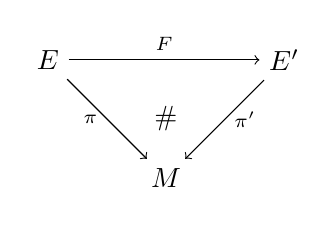
\begin{tikzpicture}
	%\draw[step=0.25,gray!15] (-6,-1) grid (6,5); \draw[step=0.5,gray!30] (-6,-1) grid (6,5); \fill (0,0) circle(0.1); %Hilfsgitter
	\node (E) at (-1.5,0.75) {$E$}; \node (E') at (1.5,0.75) {$E'$}; \node (M) at (0,-0.75) {$M$};
	
	\draw[->] (E) --node[above,font=\scriptsize]{$F$} (E');
	\draw[->] (E) --node[left,font=\scriptsize]{$\pi$} (M); \draw[->] (E') --node[right,font=\scriptsize]{$\pi'$} (M);
	
	\node at (0,0) {$\#$};
\end{tikzpicture}\end{center}

Die Vektorbündel $E,E'$ über $M$ heißen \CmMark{isomorph}, wenn ein $M$-Vektor"-bündel"-morphismus
$G$ existiert mit $G F = \Id_E$ und $FG = \Id_{E'}$.
Dies ist genau dann der Fall, wenn $F$ faserweise ein Inverses besitzt.
(Der Beweis dieser Aussage sei als Übungsaufgabe überlassen.)

Ein Vektorbündel $E \xrightarrow{\pi} M$ heißt \CmMark{trivial}, wenn es einen Vektorbündelisomorphismus von $E$ auf $M \times \R^k$ gibt. Jedes
\begin{align*}
  \tau \colon E|_U \to U \times \R^k
\end{align*}
ist ein Vektorbündelisomorphismus.
Die Bündelkarten werden daher auch \CmMark{lokale Trivialisierungen} genannt.

Es sei $(\tau_\alpha,U_{\alpha})_{\alpha \in \calI}$ eine Familie lokaler Trivialisierungen von $E$ mit $M = \bigcup_{\alpha \in J}U_{\alpha}$.
Der Diffeomorphismus
\begin{align*}
  \tau_{\alpha} \circ \tau_{\beta}^{-1}\colon (U_{\alpha} \cap U_{\beta}) \times \R^k \to (U_{\alpha} \cap U_{\beta}) \times \R^k
\end{align*}
definiert die sogenannten \CmMark{Übergangsfunktionen}
\begin{align*}
  g_{\alpha\beta} \colon U_{\alpha} \cap U_{\beta} \to \gls{GL}_k(\R)
\end{align*}
durch 
\begin{align*}
  \tau_{\alpha} \circ \tau_{\beta}^{-1}(p,x) = (p,g_{\alpha\beta}(p) x).
\end{align*}
Die Übergangsfunktionen sind glatt und für alle $p \in U_{\alpha} \cap U_{\beta} \cap U_{\gamma}$ gilt:
\begin{align*}
  g_{\alpha\gamma}(p) = g_{\alpha\beta}(p) \cdot g_{\beta\gamma}(p),
\end{align*}
denn
\begin{align*}
	(p,g_{\alpha\gamma}(p)x) & = \tau_{\alpha} \circ \tau_{\gamma}^{-1}(p,x)\\
	& = \tau_{\alpha} \circ \tau_{\beta}^{-1} \circ \tau_{\beta} \circ \tau_{\gamma}^{-1}(p,x)\\
	& = (\tau_{\alpha} \circ \tau_{\beta}^{-1})(p,g_{\beta\gamma}(p)x)\\
	& = (p,g_{\alpha\beta}(p)\cdot g_{\beta\gamma}(p)x).
\end{align*}

\begin{bsp}
  Die Übergangsfunktionen von $\T M$ sind gegeben durch
  \begin{align*}
    \D(\psi \circ \varphi^{-1}) = \left(\partial_i(\psi^j \circ \varphi^{-1})\right)_{i,j \leq m}.
  \end{align*}
\end{bsp}

% Satz 5.2
\begin{Satz}
  Es sei $M$ eine glatte Mannigfaltigkeit mit einer offenen Überdeckung $\{U_{\alpha}\}_{\alpha \in \calI}$ und einer glatten Abbildung
  \begin{align*}
    g_{\alpha\beta} \colon U_{\alpha} \cap U_{\beta} \to \Gl_k(\R)
  \end{align*}
so dass für alle $\alpha,\beta,\gamma \in \calI$ und $p \in U_{\alpha} \cap U_{\beta} \cap U_{\gamma}$ gilt:
\begin{align*}
  g_{\alpha\gamma} (p) = g_{\alpha\beta}(p)g_{\beta\gamma}(p).
\end{align*}
Dann ist
	\[ E = \bigcup_{\alpha \in \calI}^{\cdot} \FakRaum{U_{\alpha} \times \R^k}{\sim}, \]
wobei $(p,x)_{\alpha} \sim (q,y)_{\beta}$ genau dann gilt, wenn $p = q$ und $x = g_{\alpha\beta}(p)y$, ein glattes Vektorbündel.
\end{Satz}

Der Beweis sei erneut als Aufgabe überlassen.

\begin{kor}
  Ist $E$ ein glattes Vektorbündel über $M$ mit Übergangsfunktionen $\{g_{\alpha\beta}\}$, so ist das oben konstruierte Vektorbündel isomorph zu $E$.
\end{kor}

Es sei $E \xrightarrow{\pi} N$ ein Vektorbündel und $\Phi \colon M \to N$ glatt.
Das längs $\Phi$ zurückgezogene Bündel ("`\CmMark{pullback}"') ist definiert durch den Totalraum
\begin{align*}
  E' = \Phi^{\ast}E = \{(p,x) \mid x \in E_{\Phi(p)}\} \subseteq M \times E,
\end{align*}
die Projektion $\pi' \colon \Phi^{\ast}E \to M, (p,x) \mapsto p$ und die folgenden Bündelkarten:
Es sei $p \in M$ und $(\tau, U)$ eine Bündelkarte von $E$ um $\Phi(p)$, sowie $(\varphi,V)$ eine Karte von $M$ um $p$ mit $\Phi(V) \subseteq U$.
Dann definiert 
\begin{align*}
  \Phi^{\ast}E|_V \to V \times \R^k, (p,x) \mapsto \left(p, \tau_{\Phi(p)}(x)\right)
\end{align*}
eine Bündelkarte.

Sind $E \xrightarrow{\pi} M, E' \xrightarrow{\pi'} N$ Vektorbündel, dann ist $E \times E' \xrightarrow{\pi \times \pi'} M \times N$ mit lokalen Trivialisierungen $\tau \times \tau'$ ebenfalls ein Vektorbündel.
Insbesondere ist im Falle $M = N$ $E \times E'$ ein Bündel über $M \X M$.
Es sei $\Delta \colon M \to M \times M$, $p \mapsto (p,p)$.

\begin{center}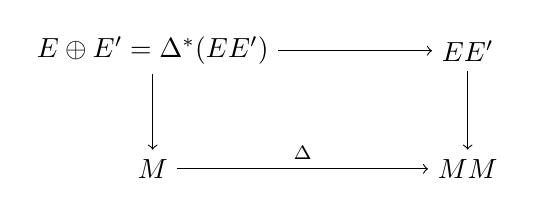
\begin{tikzpicture}
	%\draw[step=0.25,gray!15] (-6,-1) grid (6,5); \draw[step=0.5,gray!30] (-6,-1) grid (6,5); \fill (0,0) circle(0.1); %Hilfsgitter
	\node (1) at (-2,0.75) {$E \oplus E' = \Delta^*(E \X E')$}; \node (2) at (2,0.75) {$E \X E'$}; \node (3) at (-2,-0.75) {$M$}; \node (4) at (2,-0.75) {$M \X M$};
	
	\draw[->] (1) -- (2); \draw[->] (3) --node[above,font=\scriptsize]{$\Delta$} (4);
	\draw[->] (1) -- (3); \draw[->] (2) -- (4);
\end{tikzpicture}\end{center}

Das längs $\Delta$ zurückgezogene Bündel $E \oplus E' = \Delta^{\ast}(E \times E')$ heißt die \CmMark{Whitneysumme} von $E$ und $E'$.
Faserweise gilt
\begin{align*}
  (E \oplus E')_p = E_p \oplus E'_p.
\end{align*}
 
\emph{Überlege:} $\Hom(E,E')$, sowie $E \otimes E', \bigotimes E$ und $\Lambda^pE, \Lambda E$ sind "`vernünftige"' Bündel.


%%% Local Variables: 
%%% mode: latex
%%% TeX-master: "../skript-diffgeom"
%%% End: 
